% SmallSat conference LaTeX paper template based on work by Laura Yenchensky and Peter Grenfell 2018-2019.
% Updated to match original SmallSat.docx template by Rachel Morgan, March 2020.
% References to Word styles omitted, Figure 2 example added, and copy edited generally by Boyd Edwards, Utah State University, May 2020.
% Updated file organization by Ryan Thibaudeau, March 2024.
% Updated date & conference number by Ryan Martineau, April 2026

\documentclass[10pt, fleqn]{article}
\usepackage[utf8]{inputenc}
\DeclareUnicodeCharacter{2212}{$-$}
\usepackage{graphicx}
\usepackage[fleqn]{amsmath}
\usepackage[version=4]{mhchem}
\usepackage{siunitx}
\usepackage{longtable,tabularx}
\usepackage{nccmath}
\usepackage{amsmath}
\usepackage[superscript]{cite}
\usepackage[margin=1in]{geometry}
\usepackage[toc,page]{appendix}
\usepackage{setspace}
\usepackage{amssymb}
\usepackage{tabu}
\usepackage{listings}
\setlength\LTleft{0pt} 
\usepackage{afterpage}
\setlength{\columnsep}{18pt}
\usepackage{titlesec}
\usepackage[labelfont=bf]{caption}
\captionsetup{labelfont=bf,textfont=bf}
\usepackage{fancyhdr}
\usepackage{pgf}
\usepackage{float}
\usepackage{subcaption}
\usepackage{textcomp}
\usepackage{pict2e}
\usepackage{wasysym}
\usepackage{multicol}
\usepackage{lipsum}
\usepackage{indentfirst}
\usepackage{url}
\usepackage{minted}
\usepackage[pdf]{graphviz}
\usepackage{tikz}
\usepackage{pgfplots}
\usepackage{pgfplotstable}
\usepackage{hyperref}
\hypersetup{
        colorlinks,
        linkcolor={red!50!black},
        citecolor={blue!50!black},
        urlcolor={blue!80!black}
}
\newenvironment{Figure}
  {\par\medskip\noindent\minipage{\linewidth}}
  {\endminipage\par\medskip}
\newcommand\T{\rule{0pt}{2.6ex}}
\newcommand\B{\rule[-1.2ex]{0pt}{0pt}}
\pagestyle{fancy}
\fancyhead{} 
\renewcommand{\footrulewidth}{1pt}
\renewcommand{\headrulewidth}{0pt}

\pgfplotsset{compat=newest}

\usetikzlibrary{backgrounds,fadings}
\tikzfading[name=fadeout,
            inner color=transparent!0,
            outer color=transparent!100]

\usetikzlibrary{arrows.meta}

% Input the author name for the footer:
\lfoot{Curtin et al.}

\rfoot{$40^{th}$ Annual Small Satellite Conference}

\titleformat{\section}
{\normalfont\normalsize\bfseries}{\thesection}{0.5em}{}
\titleformat{\subsection}
{\normalfont\normalsize\bfseries\em}{\thesubsection}{0.5em}{}
\titleformat{\subsubsection}
{\normalfont\normalsize\bfseries\em}{\thesubsubsection}{0.5em}{}
\setlength{\mathindent}{0cm}
\newcommand\blankpage{
    \null
    \thispagestyle{empty}
    \addtocounter{page}{-1}
    \newpage
    }

\singlespacing

\begin{document}

%%%%%%%%%%%%%%%%%%%%%%%%%%%%%%%%%%%%%%%%%%%%%%%%%%%%%%%%%%%%%%%%%%%%%%%%%%%%%%%%
%%%%%%%%%%%%%%%%%%%%%%%%%%%%%%%%%%%%%%%%%%%%%%%%%%%%%%%%%%%%%%%%%%%%%%%%%%%%%%%%
%%%% TITLE %%%%
%%%%%%%%%%%%%%%%%%%%%%%%%%%%%%%%%%%%%%%%%%%%%%%%%%%%%%%%%%%%%%%%%%%%%%%%%%%%%%%%
%%%%%%%%%%%%%%%%%%%%%%%%%%%%%%%%%%%%%%%%%%%%%%%%%%%%%%%%%%%%%%%%%%%%%%%%%%%%%%%%
\begin{flushright}
\Large % (14 point font)

% Input the paper number: 
\textbf{[SSC26-VII-08]}
\end{flushright}
\begin{centering}      
\large % (12 point font)

% Input the title: 
\textbf{Lightweight Open Source On-Spacecraft Machine Learning with mlpack and \\F Prime}\\
\vspace{0.5cm}
\normalsize % set to 10 point font

% Input the author information:
Ryan R. Curtin\\
NumFOCUS, Inc.\\
\texttt{ryan@ratml.org}\\
\vspace{0.5cm}
Scott M. Gilliland\\
Georgia Institute of Technology\\
\texttt{scott.gilliland@gatech.edu}\\
\vspace{0.5cm}
Sterling L. Peet\\
Georgia Institute of Technology\\
\texttt{sterling.peet@gatech.edu}\\

\end{centering}

%%%%%%%%%%%%%%%%%%%%%%%%%%%%%%%%%%%%%%%%%%%%%%%%%%%%%%%%%%%%%%%%%%%%%%%%%%%%%%%%
%%%%%%%%%%%%%%%%%%%%%%%%%%%%%%%%%%%%%%%%%%%%%%%%%%%%%%%%%%%%%%%%%%%%%%%%%%%%%%%%
%%%% ABSTRACT %%%%
%%%%%%%%%%%%%%%%%%%%%%%%%%%%%%%%%%%%%%%%%%%%%%%%%%%%%%%%%%%%%%%%%%%%%%%%%%%%%%%%
%%%%%%%%%%%%%%%%%%%%%%%%%%%%%%%%%%%%%%%%%%%%%%%%%%%%%%%%%%%%%%%%%%%%%%%%%%%%%%%%
\begin{centering}
    \vspace{0.5cm}
    \centerline{\textbf{ABSTRACT}}
    \vspace{0.3cm}
\end{centering}

Onboard machine learning is an increasingly important topic in spaceflight systems,
as machine learning and AI models are increasingly used for
data processing, anomaly detection, attitude control systems, and other predictive applications.
However, successfully deploying a machine learning model
in a spaceflight computing environment is
fraught with difficulty,
as spaceflight computing environments are low-resource,
but typical machine learning software solutions are implemented in languages like Python,
which require an interpreter and other heavyweight dependencies.
It is therefore virtually mandatory for
any on-spacecraft machine learning
to be written with lightweight toolkits
that minimize dependencies and resource usage.

We demonstrate a solution to this problem:
via the use of open source C++-based scientific computing software,
including the mlpack machine learning library
and Armadillo linear algebra library,
we provide the first implementation of a
working on-spacecraft machine learning anomaly detection system
inside the F Prime flight software framework
that successfully detects non-trivial anomalous events
by using a kernel density estimate on telemetry data.
Our prototype is validated on real hardware,
where we physically created several anomalous situations
that were all successfully detected.
The code is available publicly on Github
and can be used as a reference project for deploying
any complex machine learning pipeline
to a spacecraft via the F Prime framework.

%%%%%%%%%%%%%%%%%%%%%%%%%%%%%%%%%%%%%%%%%%%%%%%%%%%%%%%%%%%%%%%%%%%%%%%%%%%%%%%%
%%%%%%%%%%%%%%%%%%%%%%%%%%%%%%%%%%%%%%%%%%%%%%%%%%%%%%%%%%%%%%%%%%%%%%%%%%%%%%%%
%%%% ACTUAL PAPER %%%%
%%%%%%%%%%%%%%%%%%%%%%%%%%%%%%%%%%%%%%%%%%%%%%%%%%%%%%%%%%%%%%%%%%%%%%%%%%%%%%%%
%%%%%%%%%%%%%%%%%%%%%%%%%%%%%%%%%%%%%%%%%%%%%%%%%%%%%%%%%%%%%%%%%%%%%%%%%%%%%%%%
\begin{multicols*}{2}

%%%%%%%%%%%%%%%%%%%%%%%%%%%%%%%%%%%%%%%%%%%%%%%%%%%%%%%%%%%%%%%%%%%%%%%%%%%%%%%%
\section{INTRODUCTION}
%%%%%%%%%%%%%%%%%%%%%%%%%%%%%%%%%%%%%%%%%%%%%%%%%%%%%%%%%%%%%%%%%%%%%%%%%%%%%%%%

Modern spaceflight missions
produce massive amounts of data.
NASA missions are now generating over 100~TB of data each day~\cite{lee2021nasa},
and this presents a significant challenge for data processing.
Rather than downlinking the data for ground-based processing, many are turning to 
direct on-board machine learning
to process the data~\cite{henriquez2016high, habib2022artificial, cody2017application}.
The limited computational resources available on
low-power satellites, such as CubeSats~\cite{poghosyan2017cubesat}
and other similar craft such as extraplanetary rovers
pose challenges to complex on-board processing.

Due to the focus on flight heritage for the space applications,
the chosen computational platforms of satellites can be somewhat esoteric.
Although ARM-based platforms are likely the most common,
with use in missions like SpaceCube~\cite{brewer2020nasa} and DODONA~\cite{mae2022dorbit},
legacy platforms are also in wide usage.
For instance, the ArgoMoon mission~\cite{lombardo2022design}
and Roman Space Telescope~\cite{goodwill2021nasa} use SPARC processors.
The common BAE RAD750~\cite{berger2001rad750} is a PowerPC processor and
is used on the Perserverance and Curiosity rovers~\cite{goodwill2021nasa}.
Even platforms like MIPS are in use on missions like New Horizons~\cite{kusnierkiewicz2005description}.

A further constraint on spaceflight computing systems is
the flight software framework being used to control them.
Two common choices,
both supported by NASA,
are F Prime~\cite{bocchino2018f}
and core Flight System (cFS)~\cite{mccomas2012nasa}.
cFS is written in C,
adhering to the C99 standard.
Although this allows for precise programmer control in an embedded context,
it makes interoperability with non-C99 toolkits difficult.
For similar reasons, F Prime is written in C++,
targeting the C++11 standard or newer.
The interoperability situation is better for C++,
but can still present some challenges.
Due to limited computational resources, and to reduce complexity,
it is often best to keep all computation directly in the language of the flight software toolkit.

This variety of computing platforms,
the general lack of computing resources present on them,
as well as the language limitations imposed by cFS and F Prime
present a huge barrier to
practitioners wishing to perform machine learning directly on a spacecraft.
Most widely-used machine learning software packages,
such as {\small \tt scikit-learn}~\cite{pedregosa2011scikit},
TensorFlow~\cite{abadi2016tensorflow},
or PyTorch~\cite{paszke2019pytorch}
provide interfaces in Python.
This is problematic for lightweight deployment:
Python requires a language interpreter,
which is inefficient and can be orders of magnitude larger than
storage resources permit~\cite{mlpack_pydata}.
Even projects aimed to productionalize machine learning models present problems:
efforts like XLA~\cite{sabne2020xla},
TensorFlow Lite,
and ExecuTorch for PyTorch
are cumbersome to build and link against,
as they use complex build systems and have many dependencies.
Vendor-specific alternatives like ARM's CMSIS-NN~\cite{ARM_CMSIS_NN}
suffer from limited vendor support,
limited functionality,
and cannot be deployed on other hardware.
Worse, vendor-supplied toolkits are often arbitrarily EOL'ed,
as in the case of several Qualcomm and Intel toolkits.
Another barrier encountered with these tools is complexity:
software running on-spacecraft is expected to be
highly reliable, stable, and maintainable.

Yet there exists a widely-used
native C++ scientific computing ecosystem,
made up of tools like
Armadillo~\cite{sanderson2016armadillo}, Eigen~\cite{guennebaud2010eigen}, and xTensor~\cite{xtensor} for linear algebra,
mlpack~\cite{mlpack2023}, dlib-ml~\cite{king2009dlib}, and ensmallen~\cite{curtin2021ensmallen} for machine learning,
and numerous other libraries for related tasks.
Many of these tools are intentionally lightweight, header-only, and dependency-free;
thus they can be easily cross-compiled to any target architecture
and deployed without burdensome dependency requirements.
These libraries have been deployed widely,
including for other on-board spaceflight applications~\cite{hackett2017implementation,hackett2018implementation}.

In this paper,
we put both of these pieces together to solve the problem:
we demonstrate that mlpack can be easily used inside of F Prime
to build a lightweight machine learning anomaly detector
that runs directly on-board the spacecraft
without the need for ground-based intervention.
Following Peet~et~al.~\cite{peet2024framework},
we deployed our solution to a Pololu Romi robot~\cite{PololuRomi},
which serves as a surrogate of a small satellite or extraplanetary rover.
Our anomaly detector framework was able to successfully detect
a number of complex anomalous situations
that are not trivially detected with simple methods,
e.g., thresholding.

Although our purpose here is to detect telemetry anomalies,
our solution can be trivially adapted to other common on-board machine learning tasks,
such as computer vision and image classification~\cite{giuffrida2021varphi,leon2023accelerating},
health monitoring~\cite{volponi2008enhanced},
and other tasks.
Our code is publicly available for use and adaptation at
\href{https://github.com/SterlingPeet/mlpack-fprime-robot}{\footnotesize \tt https://github.com/SterlingPeet/mlpack-fprime-robot},
licensed under the Apache license, version 2~\cite{apache2license}.
\vspace*{0.5em}

%%%%%%%%%%%%%%%%%%%%%%%%%%%%%%%%%%%%%%%%%%%%%%%%%%%%%%%%%%%%%%%%%%%%%%%%%%%%%%%%
\section{SOFTWARE OVERVIEW}
%%%%%%%%%%%%%%%%%%%%%%%%%%%%%%%%%%%%%%%%%%%%%%%%%%%%%%%%%%%%%%%%%%%%%%%%%%%%%%%%

\vspace*{-0.3em}
Our flight control software is implemented in C++ as
an F Prime deployment
that internally uses mlpack's
kernel density estimation technique
for its anomaly detection functionality.

\subsection{F Prime}
%%%%%%%%%%%%%%%%%%%%%%%%%%%%%%%%%%%%%%%%%%%%%%%%%%%%%%%%%%%%%%%%%%%%%%%%%%%%%%%%

\vspace*{-0.3em}
As mentioned earlier,
F Prime is a modular flight software framework
emphasizing the reusability of individual parts of software across different missions.
In F Prime,
each part of the flight software is
decomposed into discrete {\it Components}
with well-defined interfaces;
these serve as the fundamental building blocks
for the mission software.

A single software executable consists of a number of components
connected in a specific way,
called a {\it deployment}.
Each F Prime component's interface is defined as a
number of input and output ports,
which are defined and connected to other components.
This interface and connections are specified in the
Fpp domain-specific language~\cite{bocchino2022fpp}.
For example,
the {\small \tt Svc.SystemResources} component,
which monitors the state of the computing environment
(e.g. RAM usage, CPU utilization),
typically outputs its telemetry via an Fpp connection
to the mission telemetry service for relay to ground control systems.

The F Prime framework encapsulates all of the communication between components,
and provides numerous default components and deployments.
This means that for a user,
implementing the mission software stack
typically means taking several F Prime-supplied off-the-shelf components
and connecting them with a few custom components
implemented specifically for the mission.

Once the components are implemented
and the connections in the deployment are defined,
an F Prime deployment can easily be cross-compiled to any target platform,
including traditional platforms like VxWorks on the RAD750,
and newer platforms like ARM systems running lightweight Linux distributions
(for instance, a Raspberry Pi).

Compilation and configuration is handled via
CMake, which is likely the most widely-used C++ build system generator.
F Prime automatically generates the CMake configuration
based on the deployment topology.
A user who has implemented their flight software with F Prime
can typically build and run it with a few simple commands
via the use of the helper programs {\small \tt fprime-util} and {\small \tt fprime-gds}:

\begin{minted}{bash}
  # automatically configure CMake
  $ fprime-util generate

  # build project with CMake
  $ fprime-util build

  # run the software and display
  # ground control interface
  $ fprime-gds
\end{minted}

F Prime deployments can work even on very resource-constrained hardware;
for instance,
it has been successfully used with program memory size as small as 128 kB
and RAM as small as 64 kB~\cite{Kolhof2021,Cheek2021}.

Further resources on F Prime can be found
in the original F Prime paper~\cite{bocchino2018f}
and website~\cite{fprimewebsite},
and more details related to our deployment topology can be found
in the previous work of Peet et~al.~\cite{peet2024framework},
whose work we have used as a starting point.

\subsection{mlpack}
%%%%%%%%%%%%%%%%%%%%%%%%%%%%%%%%%%%%%%%%%%%%%%%%%%%%%%%%%%%%%%%%%%%%%%%%%%%%%%%%

mlpack is a lightweight header-only machine learning library
written in C++ with a focus on portability and efficiency~\cite{mlpack2023}.
It is built on top of the
ensmallen mathematical optimization library~\cite{curtin2021ensmallen},
the cereal serialization library~\cite{grant2017cereal},
and the well-known Armadillo linear algebra library~\cite{sanderson2016armadillo}
for its linear algebra primitives.
It can also make use of the more recent Bandicoot library~\cite{curtin2026fast}
to provide support for GPU-accelerated linear algebra operations.
All of these libraries take advantage of
C++'s template metaprogramming support
to provide significant runtime accelerations and
size reductions.

Importantly,
mlpack and all of its dependencies are header-only,
with the sole exception of Armadillo,
which must be linked against a BLAS/LAPACK library.
This significantly eases the compilation process,
as users simply need to ensure that the headers are available.
Although users must supply a compiled BLAS/LAPACK library
specific to the target architecture,
the OpenBLAS library~\cite{xianyi2012openblas} has easy support for cross-compilation
to a wide variety of targets
(including all spacecraft architectures described in the introduction),
and mlpack has a CMake-based auto-downloader that
can obtain all of the header-only dependencies of mlpack
and automatically compile or cross-compile OpenBLAS
without requiring user intervention.

From a high level,
using mlpack for machine learning purposes
is generally isomorphic to
the workflows used in Python-based toolkits such as {\small \tt scikit-learn}.
Linear algebra is performed with Armadillo (or Bandicoot),
where the API is expressly meant to mirror MATLAB
to make transition to C++ easier for researchers and practitioners.
For example, this simple code snippet creates
two random uniform matrices of size $100 \times 50$ and
computes a third as $Z = (X + Y) / 2$.

\begin{minted}{c++}
  // For more details on the Armadillo API, see
  // https://arma.sourceforge.net/docs.html.
  arma::mat X(100, 50, arma::fill::randu);
  arma::mat Y(100, 50, arma::fill::randu);
  arma::mat Z = (X + Y) / 2;
\end{minted}

Typical classification and regression algorithms in mlpack
implement a simple and unified API.
For example, supposing we wish to build a decision tree
on a dataset of observations $X$
and a vector of labels $Y$,
we can use the following code.

\begin{minted}{c++}
  // This matrix holds the predictors.
  arma::mat X;
  // This vector holds the labels.
  arma::Row<size_t> Y;

  // Create the decision tree, optionally
  // specifying parameters.
  mlpack::DecisionTree d(/* ... */);
  d.Train(X, Y);
\end{minted}

The {\small \tt d.Classify()} function could then be used to
predict the class of a new data point
using the trained decision tree.
There are also a number of hyperparameters that control the
tree-building procedure
that can be specified in the constructor,
as well as other methods that can be used to
inspect or use the tree in other ways.

Other algorithms in mlpack follow a very similar
construct-train-use paradigm,
popularized originally by {\tt \small scikit-learn}~\cite{buitinck2013api}
and roughly reflected in
virtually every modern machine learning and data science library.
Available algorithms in mlpack range from
common decision trees and logistic regression to
more specialized tree-based algorithms~\cite{curtin2013tree}
including tree-based density estimation techniques~\cite{gray2003nonparametric,ram2011density},
which is what we have chosen to use here
for our on-spacecraft anomaly detector.

It is worth noting that JPL F Prime coding conventions~\cite{jplstandards}
explicitly disallow numerous C++ features
including dynamic memory allocation after initialization.
With mlpack and related tools,
it is possible to meet each of these conventions
but extra work may be required.
For example, F Prime components that use Armadillo matrices
could either use {\tt \small arma::mat::fixed<Rows, Cols>}
to allocate a fixed-size matrix at compile time,
or could call {\tt \small mat.set\_size(rows, cols)}
at F Prime component construction time to perform dynamic allocation only once.
Other approaches exist too,
e.g., a custom allocated-once memory pool used during computation.
mlpack offers a few compile-time controls to assist with this,
including macros that allow disabling various parts of STL functionality.

\section{HARDWARE OVERVIEW}

Building on Peet et~al.~\cite{peet2024framework},
we choose the inexpensive Pololu Romi robot~\cite{PololuRomi}
(shown in Figure~\ref{fig:romi})
as a robotic explorer platform
due to its standard hardware:
an ATMega32U4-based mainboard
controlled by a Raspberry Pi via an I\textsuperscript{2}C connection;
in our case, we used a Raspberry Pi 3B+
which contains a Cortex-A53 processor at 1.4 GHz
and 1GB of RAM.
F Prime (and the machine learning anomaly detector) runs on the Raspberry Pi,
and components in the topology interact with the ATMega32U4
via I\textsuperscript{2}C.

From a control perspective,
the Romi contains two wheels with encoders for speed control,
a speaker,
and 3 LEDs (which we do not use for our work here).
From a telemetry perspective,
the following signals are available on the Romi
and can be captured for F Prime telemetry:

\begin{itemize}
  \itemsep -2pt
  \item Wheel turn counters (can be used for distance tracking)
\end{itemize} % split to fit image

\begin{Figure}
\begin{center}
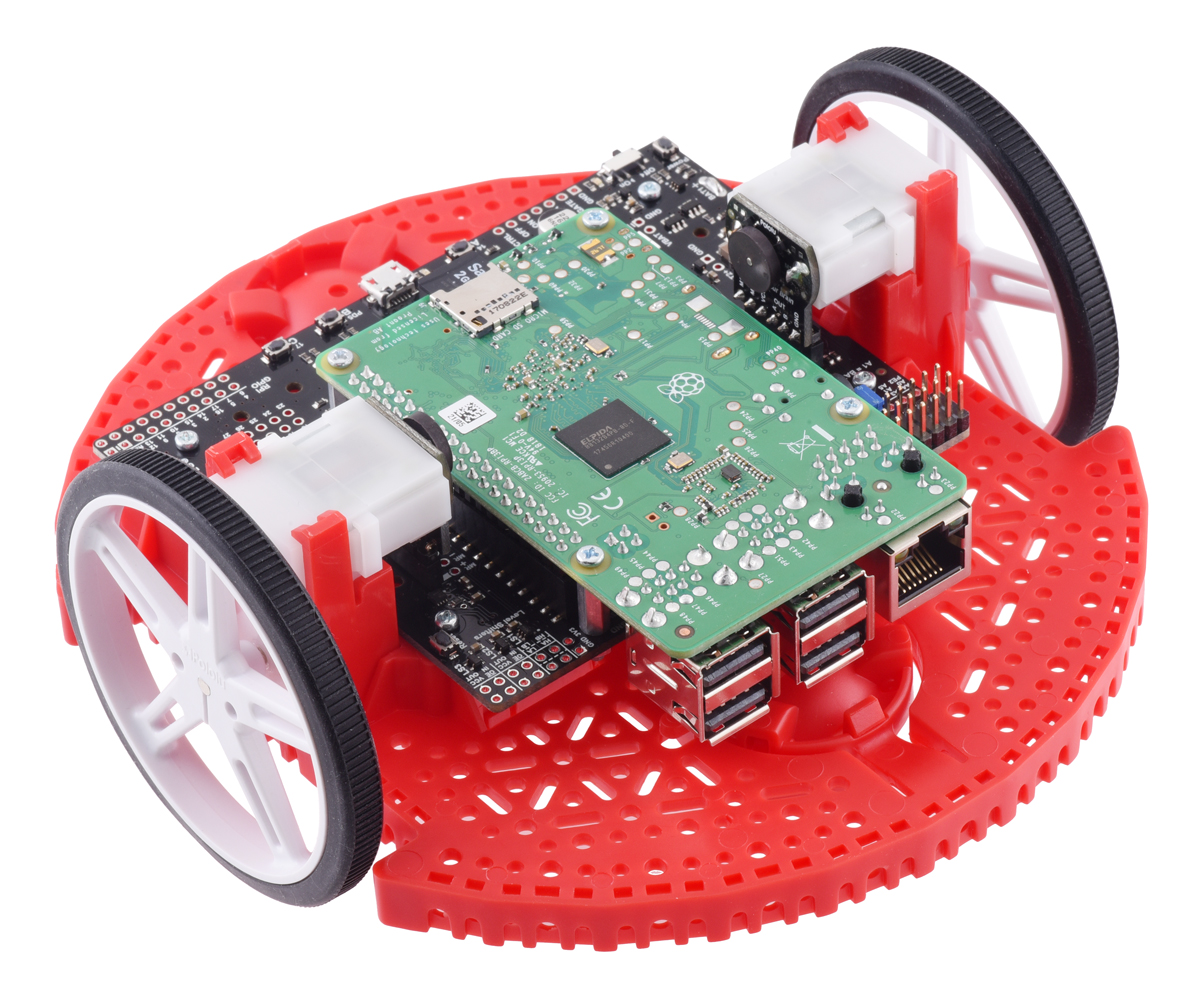
\includegraphics[width=\textwidth]{img/romi.jpg}
\end{center}
\vspace*{-1.5em}
\captionof{figure}{Pololu Romi robot.}
\label{fig:romi}
\end{Figure}

\begin{itemize}
  \itemsep -2pt
  \item Acceleration sensors (x/y/z axis)
  \item Gyrometers (x/y/z)
  \item Ambient temperature
  \item Battery level
\end{itemize}

This is in addition to the default F Prime telemetry
running on the Raspberry Pi,
which can track available memory, memory used,
and CPU utilization percentages.

Although the Romi seems unlikely to survive for very long
if deployed as-is in a spaceflight environment,
we find it to be a compelling demonstration platform,
as it reflects typical qualities of real spaceflight computing platforms:
it has limited computational power and memory,
as well as multiple interconnected devices, sensors,
and motors that enable (semi-)autonomous operation,
and its main processor architecture (ARM) is commonly used in COTS spaceflight applications.

\section{OPERATING CONCEPT}

The operating concept of our robotic explorer envisions two distinct operating settings:

\begin{itemize}
  \item {\bf Stationary}.  In this mode,
the explorer does not use its wheels to move,
and it passively collects environmental data.
It is expected in this mode that neither the
external environment (measured via temperature, acceleration)
nor the internal environment (CPU usage)
changes significantly.

  \item {\bf Straight-line}.  In this mode,
the explorer is always moving forward or backward at
any low-to-medium velocity, or is stopped.
It is expected that the measured rate of travel
matches the controlled wheel speeds,
and that the controlled and measured velocities
are not a high velocity.
\end{itemize}

During normal operation,
an anomaly detection system that tracks previous telemetry
is always running,
and should the explorer enter an operating region where the
collected telemetry does not match
telemetry collected from known-good operation,
an error will be issued.
In our implementation,
we simply used the speaker to indicate anomalies audibly.
(In a real spaceflight application,
it is likely that either a louder speaker or
some other non-acoustic anomaly reporting means would be desired.)

Commands sent to the explorer
can set it in any of these two modes,
and reset the anomaly detection system
such that its recent collected telemetry
is interpreted as corresponding to the explorer working as desired.

% F Prime Architecture for MarsRobot
\begin{Figure}
    \centering
    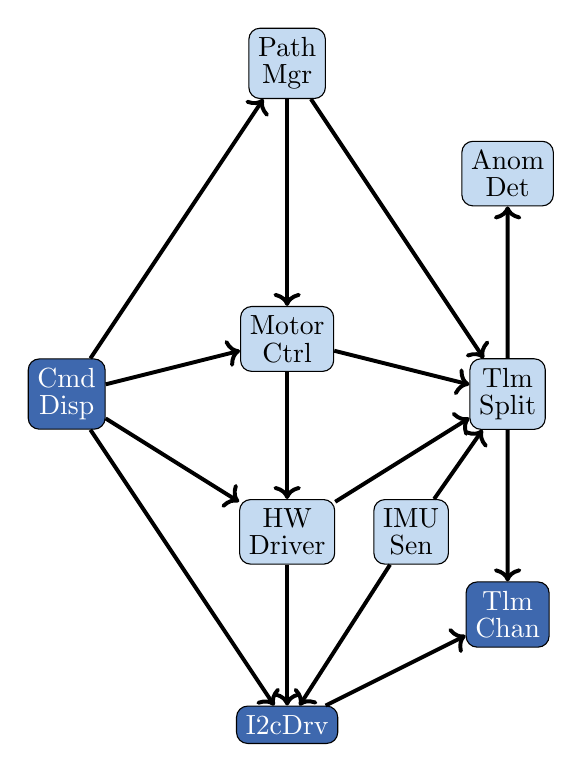
\begin{tikzpicture}[scale=0.7, every node/.style={rounded corners, draw=black}] % Adjust the scale factor as needed
        % Define the colors
        % \definecolor{yellow}{rgb}{1,1,0}
        % \definecolor{green}{rgb}{0,1,0}
        \definecolor{yellow}{HTML}{c4daf1}
        % \definecolor{green}{HTML}{527267}
        % \definecolor{green}{HTML}{252c3b} % dark?
        \definecolor{green}{HTML}{3e68ae} % dark?
        % \definecolor{green}{HTML}{b1b188}
        
        % Draw the green boxes with labels
        % \node[fill=green, text=white] (PrmDB) at (-4,-4) {\shortstack{Prm \\ DB}};
        \node[fill=green, text=white] (CmdDisp) at (-4,0) {\shortstack{Cmd \\ Disp}};
        \node[fill=green, text=white] (Event) at (4,-4) {\shortstack{Tlm \\ Chan}};
        \node[fill=yellow] (Telem) at (4,0) {\shortstack{Tlm \\ Split}};
      
        % Draw the yellow boxes with labels (center column)
        \node[fill=green, text=white] (I2CDriver) at (0,-6) {\shortstack{I2cDrv}};
        \node[fill=yellow] (RomiHWDriver) at (0,-2.5) {\shortstack{HW \\ Driver}};
        \node[fill=yellow] (RomiIMU) at (2.25,-2.5) {\shortstack{IMU \\ Sen}};
        \node[fill=yellow] (MotorCntrl) at (0,1) {\shortstack{Motor \\ Ctrl}};
        % \node[fill=yellow] (PIDCntrl) at (0,3) {\shortstack{PID \\ Ctrl}};
        \node[fill=yellow] (PathSegment) at (0,6) {\shortstack{Path \\ Mgr}};
        \node[fill=yellow] (AnomDet) at (4,4) {\shortstack{Anom \\ Det}};
      
        % Draw the arrows between center column boxes
        % \begin{scope}[transform canvas={xshift=0.7em}]
        %     \draw[->,line width=0.5mm] (I2CDriver) -- (RomiHWDriver);
        %     \draw[->,line width=0.5mm] (RomiHWDriver) -- (MotorCntrl);
        %     \draw[->,line width=0.5mm] (MotorCntrl) -- (PIDCntrl);
        %     \draw[->,line width=0.5mm] (PIDCntrl) -- (PathSegment);
        % \end{scope}
        
        % \begin{scope}[transform canvas={xshift=-0.7em}]
            \draw[->,line width=0.5mm] (RomiHWDriver) -- (I2CDriver);
            \draw[->,line width=0.5mm] (RomiIMU) -- (I2CDriver);
            \draw[->,line width=0.5mm] (MotorCntrl) -- (RomiHWDriver);
            \draw[->,line width=0.5mm] (PathSegment) -- (MotorCntrl);
            % \draw[->,line width=0.5mm] (PathSegment) -- (PIDCntrl);
        % \end{scope}
      
        % Draw the arrows from Cmd Disp to each center column box
        \draw[->,line width=0.5mm] (CmdDisp) -- (I2CDriver);
        \draw[->,line width=0.5mm] (CmdDisp) -- (RomiHWDriver);
        \draw[->,line width=0.5mm] (CmdDisp) -- (MotorCntrl);
        % \draw[->,line width=0.5mm] (CmdDisp) -- (PIDCntrl);
        \draw[->,line width=0.5mm] (CmdDisp) -- (PathSegment);
      
        % Draw the arrows from each center column box to Telem
        %\draw[->,line width=0.5mm] (I2CDriver) -- (Telem);
        \draw[->,line width=0.5mm] (RomiHWDriver) -- (Telem);
        \draw[->,line width=0.5mm] (MotorCntrl) -- (Telem);
        % \draw[->,line width=0.5mm] (PIDCntrl) -- (Telem);
        \draw[->,line width=0.5mm] (PathSegment) -- (Telem);
        \draw[->,line width=0.5mm] (RomiIMU) -- (Telem);

        \draw[->,line width=0.5mm] (Telem) -- (Event);
        \draw[->,line width=0.5mm] (Telem) -- (AnomDet);
        %\draw[->,line width=0.5mm] (AnomDet) -- (Event);
      
        % % Draw the arrows from each center column box to Event
        \draw[->,line width=0.5mm] (I2CDriver) -- (Event);
        % \draw[->,line width=0.5mm] (RomiHWDriver) -- (Event);
        % \draw[->,line width=0.5mm] (MotorCntrl) -- (Event);
        % \draw[->,line width=0.5mm] (PIDCntrl) -- (Event);
        % \draw[->,line width=0.5mm] (PathSegment) -- (Event);
      
        % % Draw the arrow from Cmd Disp to PrmDB
        % \draw[->,line width=0.5mm] (CmdDisp) -- (PrmDB);
      
       %  % Draw the arrows from each center column box to PrmDB
       %  \draw[->,line width=0.5mm] (I2CDriver) -- (PrmDB);
       %  \draw[->,line width=0.5mm] (RomiHWDriver) -- (PrmDB);
       %  \draw[->,line width=0.5mm] (MotorCntrl) -- (PrmDB);
       % . \draw[->,line width=0.5mm] (PIDCntrl) -- (PrmDB);
       %  \draw[->,line width=0.5mm] (PathSegment) -- (PrmDB);
      
    \end{tikzpicture}
    \captionof{figure}{F$^\prime$ architecture for our robotic explorer.}
    \label{fig:arch}
\end{Figure}

% \begin{figure*}[t]
% \digraph{arch}{
%   ranksep=1.0;

%   {
%     rank=same;

%     con [fillcolor=darkgoldenrod3 shape=rect label="PathMgr" style=filled fontsize=10 width=0.7];
%     mot [fillcolor=darkgoldenrod3 shape=rect label="MtrCtrl" style=filled fontsize=10 width=0.7];
%     kde [fillcolor=darkgoldenrod3 shape=rect label="AnomDet" style=filled fontsize=10 width=0.7];
%     rhw [fillcolor=darkgoldenrod3 shape=rect label="HWDrv" style=filled fontsize=10 width=0.7];
%     rim [fillcolor=darkgoldenrod3 shape=rect label="IMUSen" style=filled fontsize=10 width=0.7];
%     i2c [fillcolor=darkgoldenrod3 shape=rect label="I2cDrv" style=filled fontsize=10 width=0.7];
%   }

%   {
%     rank=same;

%     tlms [fillcolor=darkgoldenrod3 shape=rect label="TlmSplit" style=filled fontsize=10 fixedsize=true width=1.2];
%     blank [label="" shape=plaintext width=0.3];
%     tlm [fillcolor=chartreuse4 shape=rect label="TlmChan" style=filled fontsize=10 fixedsize=true width=1.1];
%   }

%   tlms -> blank [style=invis];
  
%   con -> mot;
%   mot -> kde;
%   kde -> rhw;
%   mot -> rhw;
%   mot -> rim;
%   rhw -> i2c;

%   con -> tlms;
%   mot -> tlms;
%   kde -> tlms;
%   rhw -> tlms;
%   rim -> tlms;

%   tlms -> tlm;
%   tlms -> kde;
%   i2c -> tlm;
% }
% \vspace*{-5em}
% \captionof{figure}{F Prime component topology for our robotic explorer.}
% \label{fig:arch}
% \end{figure*}

\section{ARCHITECTURE}

In order to support the two modes of operation desired for our robotic explorer,
we architect F Prime components as shown in Figure~\ref{fig:arch}.
Each component already provided by F Prime is printed in dark blue,
while components developed specifically for our mission requirements are in light blue.
A few less important connections between components are omitted for brevity.
A description of each component's responsibilities is below:

% TODO: some of these still need descriptions!
\begin{itemize}
  \item {\bf CmdDisp}: dispatches incoming operator commands to the relevant components; included in F Prime.
  \item {\bf PathMgr}: overall control; issues commands to put the explorer in one of the two path modes.
  \item {\bf MotorCtrl}: motor control; sets the motor speeds and computes odometry.  \item {\bf AnomDet}: density-estimation anomaly detector implemented with mlpack; receives telemetry from TlmSplit.
  \item {\bf HWDriver}: Romi hardware driver; issues hardware commands via I2cDrv to I\textsuperscript{2}C.
  \item {\bf IMUSen}: Romi IMU sensor driver; issues hardware commands via I2cDrv to I\textsuperscript{2}C.
  \item {\bf I2cDrv}: low-level I\textsuperscript{2}C driver included in F Prime.
  \item {\bf TlmSplit}: telemetry splitter; routes all telemetry {\em both} to default TlmChan and also AnomDet.
  \item {\bf TlmChan}: telemetry collector included in F Prime.
\end{itemize}

Note that because F Prime restricts outputs from components to be routed to only one destination component,
we implemented a telemetry splitter (TlmSplit)
with one input port for input telemetry
and two output ports.
This allows us to duplicate all telemetry to both the default F Prime telemetry system
and our custom anomaly detector.

\section{ANOMALY DETECTION}

\begin{figure*}[t]
\begin{center}
\begin{tikzpicture}[scale=1.6]

  \draw[->,thick] (-0.3,0) -- (6,0);
  \draw[->,thick] (0,-0.3) -- (0,4);

  \begin{scope}[on background layer]
    \foreach \p in {(2.2,2.0), (3.0,2.8), (2.6,1.4), (3.6,1.8)} {
      \shade[shading=radial,
             inner color=blue!80,
             outer color=blue!80,
             opacity=0.60,
             path fading=fadeout]
        \p circle (1.4);
    }
  \end{scope}

  \foreach \p in {(2.2,2.0), (3.0,2.8), (2.6,1.4), (3.6,1.8)}
    \fill[blue] \p circle (2.5pt);

  \fill[red] (2.9,2.1) circle (2.5pt);
  \node[black,anchor=south west] at (2.95,2.15) {\small $q_1$ (high density)};

  \fill[red] (5.0,3.0) circle (2.5pt);
  \node[black,anchor=south west] at (5.05,3.05) {\small $q_2$ (low density)};

\end{tikzpicture}

\end{center}
\vspace*{-0.5em}
\captionof{figure}{Kernel density estimation.
The observed telemetry points (blue) are used to model the distribution (also blue)
via convolution with a Gaussian kernel.
Then, new telemetry points are compared with the distribution (red).
Point $q_2$ is outside the distribution and may be considered an anomaly.}
\label{fig:kde}
\end{figure*}

Historically,
anomaly detection was performed on spacecraft via
simple thresholds applied to telemetry values~\cite{fuertes2016improving}.
However, this simple approach suffers from many false positives,
needs tedious and error-prone tuning of the thresholds,
and cannot easily detect situations where each individual telemetry value
is within tolerance, but combinations of values indicate a malfunction.
(Consider, as we will later, the trivial case of a wheel's rate of motion
not matching the power applied to it.)

Of course,
more recent efforts have used far more complex techniques to detect anomalies,
including
LSTMs (neural networks)~\cite{hundman2018detecting},
convolutional neural networks~\cite{liu2023spacecraft},
and kernel methods~\cite{fujimaki2005approach},
to name a few.
Of note is that the majority of these efforts are applying machine learning on the ground,
instead of directly on the spacecraft.

With F Prime and mlpack,
each of the techniques referenced above (and many more)
can be deployed and run directly on the spacecraft,
presuming that the spacecraft has the computational power necessary to run the technique.
For `traditional' machine learning techniques like a decision tree this is not generally a problem,
but neural-network based approaches such as LSTMs
can have much higher computational requirements,
depending on the size of the network being used.

Because our efforts here are to demonstrate a working prototype,
we opt to keep our machine learning simple and easy to understand.
We will use a kernel density estimation (KDE) approach to
model the probability density of observed telemetry states.
Then, the anomaly detection system will
compute the probability of the current telemetry state,
and if that probability is exceedingly low,
then the system concludes that we are in an anomalous state
and emits an audible error tone via the buzzer.

This approach is best described visually,
as in Figure~\ref{fig:kde}.
Due to the limitations of the medium,
the figure can only show the density estimate in two dimensions;
however, as we are receiving numerous channels of telemetry from various components,
our density estimator as implemented uses 31 dimensions of telemetry.
As this is a demonstration,
we manually tune the density limit used to classify as an anomaly.
In a real-world application that used this approach,
the density should be tuned by collecting large amounts of non-anomalous data
and building an accurate model of the distribution.

% Needs to be way up high to get into the right place.
\begin{figure*}[t]
\begin{center}
\begin{tikzpicture}
\begin{axis}
  [
  width=\textwidth,
  height=0.2\textwidth,
  title=CPU utilization,
  axis y line=left,
  axis x line=bottom,
  xticklabel=\empty,
  ytick={0,50,100},
  ]
  \addplot
      [
        no markers,
        color=blue
      ]
      table
      [
        x=row,
        y=cpu00,
        col sep=comma
      ]
      {data/stationary_short.csv};
\end{axis}
\end{tikzpicture}
\begin{tikzpicture}
\begin{axis}
  [
  width=\textwidth,
  height=0.2\textwidth,
  title=Log-density estimate,
  axis y line=left,
  axis x line=bottom,
  xlabel=Time (s),
  ymin=-40,
  ytick={-40,-20,0},
  yticklabels={\ \ \ -40,-20,0} % spaces for alignment
  ]
  \addplot
      [
        no markers,
        color=red
      ]
      table
      [
        x=row,
        y=logdensityestimate,
        col sep=comma
      ]
      {data/stationary_short.csv};
\end{axis}
\end{tikzpicture}
\end{center}
\vspace*{-1.5em}
\captionof{figure}{CPU telemetry over time for stationary operation and
log-density estimates for anomaly detector.
Both manual anomalies were easily detected,
when the log-density estimate dropped noticeably for more than five seconds.}
\label{fig:stationary_telem}
\end{figure*}

Implementationally speaking,
mlpack's {\small \tt KDE} class is used to model the distribution.
Internally, mlpack uses tree-based algorithms~\cite{gray2003nonparametric}
to provide an efficient estimate of the density for a given telemetry point.
To keep the tree small on a low-resource spacecraft,
we use a configurable moving window of historical telemetry
to model the probability density.

We tuned our density estimator to use
a Gaussian kernel with bandwidth of $0.38$
and used a simple threshold of $-20$ for the log-density estimate
to identify an anomaly.
A real-world application of this technique might
cross-validate the bandwidth selection,
and use labeled anomalies to tune the threshold;
but for our purposes
(a software deployment demonstration)
we do not find that necessary.

\section{EXPERIMENTS}

In order to validate our approach,
we cross-compiled and deployed our F Prime flight software stack
on the rover
(using {\small \tt fprime-util generate aarch64-linux} and {\small \tt fprime-util build aarch64-linux})
and performed a series of real-world experiments,
verifying that the anomaly detection system
worked successfully in each anomalous situation we created.

\subsection{Stationary Operation}

As a first test of the system,
we trained the density estimate
on $10$k samples of data
where the robot was entirely stationary
and receiving no commands.
During this time,
because the robot was idle,
all motor and odometry sensors read zero
and CPU usage was minimal.

Once the density estimate was trained,
we observed the system functioning without spurious anomaly detections for
a few hours.
(Our implementation performs anomaly checks at $1$ Hz.)
Then, we twice launched computationally intensive tasks
on the Raspberry Pi.
Each time we did this,
the anomaly detection system easily detected the situation and emitted audible alerts,
as expected.

\begin{Figure}
\begin{center}

\includegraphics[width=0.92\textwidth]{img/romi_anomaly.png}
\end{center}
\vspace*{-1em}
\captionof{figure}{An anomalous situation the rover may encounter in straight-line operation.}
\label{fig:straight_anomaly}
\end{Figure}

Telemetry for CPU1 utilization and the log-density estimate are shown in Figure~\ref{fig:stationary_telem}.
The two anomalous situations are plainly obvious from the telemetry log;
the log-density estimates drop significantly.
An interesting observation is the robustness of the density estimator:
because we trained it on a few hours of real-world telemetry data,
the slightly higher CPU usage before the first anomaly is not itself detected as an anomaly,
since this level of CPU usage was regularly seen during the training period,
due to e.g. background system services running on the Raspberry Pi.

\begin{figure*}[t!]
\begin{center}
\begin{tikzpicture}
\begin{axis}
  [
  width=\textwidth,
  height=0.2\textwidth,
  title=Target wheel speed,
  axis y line=left,
  axis x line=bottom,
  xticklabel=\empty,
  ymin=-300,
  ymax=300,
  ytick={-300,0,300},
  yticklabels={-max,0,max}
  ]
  \addplot
      [
        no markers,
        color=blue
      ]
      table
      [
        x=row,
        y=left_speed,
        col sep=comma
      ]
      {data/straight.csv};

  \addplot
      [
        no markers,
        color=blue
      ]
      table
      [
        x=row,
        y=right_speed,
        col sep=comma
      ]
      {data/straight.csv};
\end{axis}
\end{tikzpicture}
\begin{tikzpicture}
\begin{axis}
  [
  width=\textwidth,
  height=0.2\textwidth,
  title=Observed wheel velocity,
  axis y line=left,
  axis x line=bottom,
  xticklabel=\empty,
  ymin=-5000,
  ymax=5000,
  ytick={-5000,0,5000},
  yticklabels={-max,0,max}
  ]
  \addplot
      [
        no markers,
        color=green!60!black
      ]
      table
      [
        x=row,
        y=left_velocity,
        col sep=comma
      ]
      {data/straight.csv};

  \addplot
      [
        no markers,
        color=green!60!black
      ]
      table
      [
        x=row,
        y=right_velocity,
        col sep=comma
      ]
      {data/straight.csv};
\end{axis}
\end{tikzpicture}
\begin{tikzpicture}
\begin{axis}
  [
  width=\textwidth,
  height=0.2\textwidth,
  title=Z-axis acceleration,
  axis y line=left,
  axis x line=bottom,
  xticklabel=\empty,
  ytick={-1,0,1},
  yticklabels={\ \ \ \ -1,0,1} % spacing for alignment
  ]
  \addplot
      [
        no markers,
        color=brown
      ]
      table
      [
        x=row,
        y=accel_z,
        col sep=comma
      ]
      {data/straight.csv};
\end{axis}
\end{tikzpicture}
\begin{tikzpicture}
\begin{axis}
  [
  width=\textwidth,
  height=0.2\textwidth,
  title=Log-density estimate,
  axis y line=left,
  axis x line=bottom,
  ymin=-50,
  xticklabel=\empty,
  ytick={-40,-20,0},
  yticklabels={\ \ \!-40,-20,0} % spacing for alignment
  ]
  \addplot
      [
        no markers,
        color=red
      ]
      table
      [
        x=row,
        y=logdensityestimate,
        col sep=comma
      ]
      {data/straight.csv};
\end{axis}

\draw [>-Stealth] (2.5, -0.3) -- (3.6, 0.5);
\node [] at (2.5, -0.5) { speed too fast };

\draw [>-Stealth] (6.0, -0.3) -- (7.3, 0.75);
\node [] at (6.0, -0.5) { both wheels obstructed };

\draw [>-Stealth] (8.5, -0.7) -- (8.75, 0.32);
\node [] at (8.5, -0.9) { one wheel obstructed };

\draw [>-Stealth] (9.5, -0.3) -- (10.1, 0.4);
\node [] at (10.2, -0.5) { rover upside-down };

\draw [>-Stealth] (12.4, -0.7) -- (12.4, 0.6);
\node [] at (12.4, -0.9) { rover on one side };

\draw [>-Stealth] (14.4, -0.3) -- (13.7, 0.6);
\node [] at (14.4, -0.5) { rover in the air };
\end{tikzpicture}
\end{center}
\vspace*{-1.0em}
\captionof{figure}{Partial telemetry and log-density estimates for
straight-line mode anomaly detection.
We applied six different anomalies,
each of which caused the log-density estimates to plummet.}
\label{fig:straight_telem}
\end{figure*}

\subsection{Straight-line Operation}

The next mode of operation we tested was straight-line operation.
In this mode of operation,
the rover is expected to be moving forward or backward at low-to-medium speeds.
Because the density estimate is trained on `normal' telemetry,
where `normal' is with respect to the mode of operation,
we ran the rover in a clean environment with no obstructions or other problems
for approximately 30 minutes.
During this time,
the rover's speed was set to alternating positive and negative speed values,
eventually cycling through all accepted speed values.
This process enables the density estimate to properly model
all regions of the operating space.

Once the training process was complete,
we operated the rover in straight-line mode,
setting a variety of different target wheel speeds
over time.
We also applied six different anomaly conditions:

\begin{enumerate}
  \itemsep -2pt
  \item Setting the speed outside the operating region's bounds
  \item Obstructing both wheels completely (no movement)
  \item Obstructing only one wheel completely
  \item Picking up the rover and turning it upside down
  \item Picking up the rover and setting it on its side
  \item Holding the rover in the air
\end{enumerate}

Figure~\ref{fig:straight_telem} shows the telemetry and density estimate
over this period
for a few of the numerous sensors that are connected to the density estimator.
In each anomalous situation,
the log-density estimate drops precipitously,
as expected.
Note that the last anomaly (rover in the air)
isn't clearly captured by the displayed sensors in the figure;
other telemetry values going outside the norm caused the drop in the density.

Overall, these successful detections validate our approach.
Although kernel density estimation is not the most powerful known anomaly detector,
our aim was simply to demonstrate a working machine learning-based anomaly detection system
that was capable of running directly on the spacecraft.
Using more complex techniques is left as future work;
for now, our publicly available code can be easily used as a starting point.

\section{CONCLUSION}

We have demonstrated an approach for on-spacecraft machine learning
in a resource-efficient and simple way
by pairing the F Prime flight software framework with
the lightweight mlpack C++ machine learning library.
The architecture of F Prime allows an easy way to
isolate the machine learning functionality specifically in its own components,
meaning that it is easy to drop in place into existing F Prime projects.

In our experiments,
we used a simple density estimator to detect anomalies
and validated that the mlpack-based model was able to
successfully run and detect anomalies
on real-world low-resource hardware
that might be used in spaceflight missions.

Because mlpack and F Prime are both easy to cross-compile to
any target architecture,
it would be trivial to recompile our project
for, e.g., SPARC64, MIPS, or PowerPC.

Future work to deploy an approach like this to a real-world mission would include
adapting parts of mlpack and Armadillo code to follow
the JPL style guidelines~\cite{jplstandards},
and implementing a more robust machine learning-based anomaly detection system.

Our code is publicly available at
\href{https://github.com/SterlingPeet/mlpack-fprime-robot}{\footnotesize \tt https://github.com/SterlingPeet/mlpack-fprime-robot}
and is licensed under the Apache license, version 2.0.
Telemetry logs of our experiments
(and the source code for this paper)
are all included in the repository.

\end{multicols*}
\bibliography{refs}
\bibliographystyle{unsrt}


\end{document}

